\documentclass[]{book}
\usepackage{lmodern}
\usepackage{amssymb,amsmath}
\usepackage{ifxetex,ifluatex}
\usepackage{fixltx2e} % provides \textsubscript
\ifnum 0\ifxetex 1\fi\ifluatex 1\fi=0 % if pdftex
  \usepackage[T1]{fontenc}
  \usepackage[utf8]{inputenc}
\else % if luatex or xelatex
  \ifxetex
    \usepackage{mathspec}
  \else
    \usepackage{fontspec}
  \fi
  \defaultfontfeatures{Ligatures=TeX,Scale=MatchLowercase}
\fi
% use upquote if available, for straight quotes in verbatim environments
\IfFileExists{upquote.sty}{\usepackage{upquote}}{}
% use microtype if available
\IfFileExists{microtype.sty}{%
\usepackage{microtype}
\UseMicrotypeSet[protrusion]{basicmath} % disable protrusion for tt fonts
}{}
\usepackage{hyperref}
\hypersetup{unicode=true,
            pdftitle={Physics for Introductory Biology},
            pdfauthor={Jeffrey A. Walker},
            pdfborder={0 0 0},
            breaklinks=true}
\urlstyle{same}  % don't use monospace font for urls
\usepackage{natbib}
\bibliographystyle{apalike}
\usepackage{longtable,booktabs}
\usepackage{graphicx,grffile}
\makeatletter
\def\maxwidth{\ifdim\Gin@nat@width>\linewidth\linewidth\else\Gin@nat@width\fi}
\def\maxheight{\ifdim\Gin@nat@height>\textheight\textheight\else\Gin@nat@height\fi}
\makeatother
% Scale images if necessary, so that they will not overflow the page
% margins by default, and it is still possible to overwrite the defaults
% using explicit options in \includegraphics[width, height, ...]{}
\setkeys{Gin}{width=\maxwidth,height=\maxheight,keepaspectratio}
\IfFileExists{parskip.sty}{%
\usepackage{parskip}
}{% else
\setlength{\parindent}{0pt}
\setlength{\parskip}{6pt plus 2pt minus 1pt}
}
\setlength{\emergencystretch}{3em}  % prevent overfull lines
\providecommand{\tightlist}{%
  \setlength{\itemsep}{0pt}\setlength{\parskip}{0pt}}
\setcounter{secnumdepth}{5}
% Redefines (sub)paragraphs to behave more like sections
\ifx\paragraph\undefined\else
\let\oldparagraph\paragraph
\renewcommand{\paragraph}[1]{\oldparagraph{#1}\mbox{}}
\fi
\ifx\subparagraph\undefined\else
\let\oldsubparagraph\subparagraph
\renewcommand{\subparagraph}[1]{\oldsubparagraph{#1}\mbox{}}
\fi

%%% Use protect on footnotes to avoid problems with footnotes in titles
\let\rmarkdownfootnote\footnote%
\def\footnote{\protect\rmarkdownfootnote}

%%% Change title format to be more compact
\usepackage{titling}

% Create subtitle command for use in maketitle
\providecommand{\subtitle}[1]{
  \posttitle{
    \begin{center}\large#1\end{center}
    }
}

\setlength{\droptitle}{-2em}

  \title{Physics for Introductory Biology}
    \pretitle{\vspace{\droptitle}\centering\huge}
  \posttitle{\par}
    \author{Jeffrey A. Walker}
    \preauthor{\centering\large\emph}
  \postauthor{\par}
      \predate{\centering\large\emph}
  \postdate{\par}
    \date{2020-02-15}

\usepackage{booktabs}
\usepackage{amsthm}

\makeatletter
\def\thm@space@setup{%
  \thm@preskip=8pt plus 2pt minus 4pt
  \thm@postskip=\thm@preskip
}
\makeatother

\begin{document}
\maketitle

{
\setcounter{tocdepth}{1}
\tableofcontents
}
\chapter{Physics for Introductory
Biology}\label{physics-for-introductory-biology}

\section{Scalar and vector
quantities}\label{scalar-and-vector-quantities}

If a measure has magnitude only, it is a \textbf{scalar quantity}. If a
measure has a magnitude and a direction, it is a \textbf{vector
quantity}. A scalar more generally is a single number. A vector more
generally is a column (or row) of numbers. A vector is called a vector
because the column of numbers can be represented by an arrow from the
origin to the point in space with coordinates equal to each number in
the column. The magnitude is the length of the arrow. The direction is
the direction of the arrow. In physics, a vector quantity is 2-D -- it's
a column of two numbers. In \emph{Physics for Introductory Biology}, the
two numbers are magnitude and direction. For example, the
electrochemical ``driving force'' of an ion is a vector quantity with a
magnitude voltage and a direction of ``in'' or ``out'' of the cell.

\section{Concepts of motion}\label{concepts-of-motion}

\textbf{displacement} is the change of position of an object. This
change includes a distance and a direction so it is a \textbf{vector}
quantity. For example. If I'm measuring the flow of labeled water in
xylem sap, I'll measure the labelled water at two points in time. The
displacement is the distance traveled in the direction of the flow.

\textbf{Velocity} is the change in displacement over time. So in our
example the xylem sap moved 9.8 cm during the measured time period,
which is 60 s, so the velocity .16 cm s\(^{-1}\). Velocity is a vector
quantity, meaning there is a magnitude component, which is also called
speed, and a directional component. So xylem flowing up a tree at .16 cm
s\(^{-1}\) and phloem flowing down a tree at .16 cm s\(^{-1}\) have
different velocities but the same speed. This comparison seems absurd
because all we care about is the speed in this comparison, which is the
same for the xylem and phloem. But direction (and so velocity) does
matter in many physiological comparisons. If you walk in a straight line
at 8 miles per hour or you walk in a circle with a radius of 2 feet at 8
miles per hour than your velocity is not changing in the first but is in
the second. Your inner ear senses this change in velocity and is the
first step in you becoming dizzy.

\textbf{Acceleration} is the change in velocity over time. Your inner
ear contains an organ that functions as an accelerometer. We cannot
sense velocity - inside a plane I cannot tell if the plane is sitting on
the tarmac or flying at 500 mph - but we can sense change in velocity
(or acceleration). Acceleration also is a vector quantity. Importantly,
in everyday language we use ``accelerate'' to mean ``getting faster''
and ``decelerate'' to mean ``slowing down'', but in science ``getting
faster'' is positive acceleration and ``slowing down'' is negative
acceleration (that is, a negative number), and this is \emph{always}
with respect to some direction.

\textbf{Jerk} is the change in acceleration over time. We won't talk
about jerk!

\section{Concepts of density, mass, inertia, force,
momentum}\label{concepts-of-density-mass-inertia-force-momentum}

The \textbf{density} of an object is how much the space bound by the
object is filled with matter (atoms). The closer the atoms or molecules
in the object are to each other, the less ``nothing'' there is and the
more dense the object. A box of air isn't very dense because air is a
collection of gas molecules that are relatively far apart with nothing
in between. A rock is more dense than air because the atoms that make up
the minerals in the rock are all bound closely together.

There are two ways to define \textbf{mass}. The material definition of
mass is a measure of the total amount of matter in an object (where
density is a per volume measure), so this is the density times the
volume\footnote{\(M=\rho V\)}, where \(\rho\) (the greek letter
\emph{rho}) is density. The inertial definition is: mass is the property
of an object that resists acceleration (this property is
\textbf{inertia}). This way of thinking about mass blew my mind when I
learned it, because it is much more useful in functional biology. To
understand the inertial definition, we need to know what makes an object
accelerate, which is a force.

A \textbf{force} is the something applied to an object that potentially
causes the object to accelerate. A force isn't necessary for an object
to move. A force applied to an object slows it down or speeds it up. So
blood moving through an artery is slowed down by friction (a type of
force) and speeded up by the heart pressurizing the blood (another kind
of force).

Newton's second law states that force is the product of mass times
acceleration\footnote{\(F=MA\)}. We can re-arrange this to
\(A=\frac{F}{M}\). Given the same force applied to two objects, the more
massive object (bigger \(M\)) will have a smaller acceleration. So this
is the inertial definition of mass: mass is the property of an object
that resists acceleration. This concept leads directly to the concept of
momentum.

\textbf{Momentum} is the mass of an object times its velocity\footnote{\(p = M\nu\)},
where \(\nu\) is the greek letter \emph{nu}. We usually think of
momentum as we would inertia: an object with more momentum resists
change in direction and/or speed more than an object with less momentum.
But it's really the mass (inertial) component of momentum that makes
this so.

Finally, note that the change in momentum over time is
\(\frac{\Delta M \nu}{T} = M \frac{\Delta \nu}{T} = MA = F\)! That is,
force is the change in momentum over time.

\section{Energy and power}\label{energy-and-power}

Energy is a very elusive concept but here are a couple of notes. First,
energy is never created or destroyed, it just changes from one form to
another and this really is the story of much of science, including
biology. One form of energy is called \textbf{mechanical energy} and
it's the energy of doing \textbf{work} where work is the energy
necessary to \textbf{displace} an object over some distance. Work is
equal to the force applied to the object times the distance the object
moves\footnote{\(W=FD\)}. A tree has to use energy to move xylem sap up
its trunk and we say that it ``does work on the xylem''. This work
(mechanical energy) is the force applied to the xylem times the distance
the xylem moves. The longer the distance the more work (given the same
force). Another form of energy is \textbf{kinetic energy} which is the
energy of a moving object, and is one-half of the product of the
object's mass and velocity squared\footnote{\(KE = \frac{1}{2}MV^2\)}.
When a cheetah runs, its hand and foot impact the ground with a certain
amount of kinetic energy which suddenly goes to zero so this energy is
transferred into the skeleton of the limbs. The cheetah will want a
skeleton that can absorb and release this energy without permanently
deforming or breaking the skeleton! Another form of energy is
\textbf{potential energy} which is the \emph{capacity to do work}. huh?
A way of thinking about this is, potential energy isn't doing anything
but it can! When it does, the potential energy is converted to some
other form of energy. Potential energy comes in several forms. It could
be the energy of an elevated mass in a gravitational field. Gravity
makes the mass fall, which transfers this potential energy to kinetic
energy. Or it could be the electrochemical energy in an ion gradient,
such as the H\(^+\) gradient in a mitochondria. The potential energy of
the H\(^+\) gradient is transferred into the kinetic energy of the ATP
synthase mechanism which is then transferred into the potential energy
of the phosphate bond in ATP. Or it could be the elastic strain energy
stored in the myosin head. We will talk a lot about this kind of energy
transfer.

\textbf{Power} is the rate of working or the rate that energy is used,
so is equal to the Work divided by the time spent doing the
work\footnote{\(P=\frac{W}{T}\)}. It takes about the same amount of
energy (work) for a cheetah to walk or to run a mile but the running
cheetah expends this energy over a much shorter amount of time so
running requires more Power. Note that since \(W=FD\) then
\(P=F\frac{D}{T} = F\nu\), that is power is the product of force and
velocity\footnote{\(P=F\nu\)}. So high power activities are activities
with high force at a high velocity or done over a short amount of time.

\chapter{Water}\label{water}

\section{The reason for everything}\label{the-reason-for-everything}

\begin{enumerate}
\def\labelenumi{\arabic{enumi}.}
\tightlist
\item
  polar covalent bonds between O and H create an asymmetric distribution
  of electrons in a water molecule -- with two excess electrons on the O
  side of the molecule and two deficient electrons on the hydroden side.
\item
  This asymmetry gives water molecules the property of 1) cohesion --
  the attraction of water molecules to other water molecules and 2)
  adhesion -- the attraction of water molecules to substances that are
  charged or have charge asymmetries including ions, polarized
  molecules, and charged surfaces such as glass.
\end{enumerate}

\section{Consequences}\label{consequences}

\subsection{Lakes don't freeze because, as water cools, it becomes more
dense, until it
doesn't}\label{lakes-dont-freeze-because-as-water-cools-it-becomes-more-dense-until-it-doesnt}

\subsection{Water is a pretty good
solvent.}\label{water-is-a-pretty-good-solvent.}

\subsection{Heat Capacity}\label{heat-capacity}

\subsection{Water is stiff in
compression}\label{water-is-stiff-in-compression}

\subsection{Humans regulate body temperature using evaporative
cooling}\label{humans-regulate-body-temperature-using-evaporative-cooling}

The temperature of a system is the average kinetic energy of the
particles in the system. Remember that \(KE = \frac{1}{2}MV^2\), where
\(M\) is mass and \(V\) is speed. Water is liquid because the \(KE\) of
the water molecules is small enough that the molecules arethey are able
to interact and form hydrogen bonds. This keeps the water molecules
relatively close to each other. By contrast water vapor (water molecules
in a gas phase) have too much kinetic energy to interact and form
hydrogen bonds. In air, water molecules are far apart. Because water
molecules in the liquid phase are highly attracted to each other, water
has a high heat of vaporization, which means it takes a relatively large
amount of energy to transition the water from a liquid to gas phase
(``Heat'' is a form of energy not a measure of temperature).

If heat energy is transferred into water, the average \(KE\) (and
therefore, temperature) increases. With enough heat transfer, the
fastest water molecules will have enough \(KE\) that they cannot
interact with other water molecules and they evaporate from the surface
as water vapor -- that is, they have transitioned from a liquid to a gas
phase. Because the water molecules that evaporate are the molecules with
the highest \(KE\), the average \(KE\) of the remaining water is
lowered. The opposite occurs as heat is transferred out of moist air.
The average \(KE\) of the water molecules decreases and water molecules
are, on average, closer together (the relative humidity increases). If
enough heat is transferred out, the water moleculees with the smallest
\(KE\) can interact with each other forming hydrogen bonds and
condensing into liquid drops. The result is rain, clouds, and fog. If a
cold surface cools the air at it's surface, the result is condensation.

Humans and other mammals generate a tremendous amount of heat from the
many chemical reactions that occur in our cells. This heat maintains our
body temperature well above that of our surrounding environment. When
skeletal muscles are working at a high rate (high \textbf{power}), they
generate excess heat, which increases the average \(KE\) of the water
(and other) molecules in the body. In humans, sweat glands are
stimulated to secrete water onto the surface. The water molecules in the
sweat with the highest \(KE\) evaporate as long as the air is not
saturated with water vapor. This evaporation lowers the average \(KE\)
(and thus temperature) of the remaining water in the body. And because
water's high heat of vaporization, this evaporation is a very effective
mechanism for cooling. Sweat glands are a highly unusual, but very
effective, method of cooling in mammals.

Sweating only cools if water \emph{can} evaporate from the surface --
sweating itself doesn't cool the body. This means that as air becomes
more saturated with water vapor (that is, increased relative humdity),
water is less likely to evaporate because the there is less and less
more ``room'' in the air for water molecules. High relative humdity is
not just a function of the east coast of the U.S. in the summer.
Evaporation from a human running on a treadmill in a closed room with
poor ventillation and air circulation can rapidly increase the relative
humidity of the air surrounding their body and decrease the
effectiveness of evaporative cooling.

\subsection{Water has high surface
tension}\label{water-has-high-surface-tension}

Consider a sheet of rubber. If I pull on a rubber sheet, I transfer
mechanical energy into sheet and stretch the material (literally pulling
atoms further apart). The stretched atomic structure of the rubber
material resists being stretched -- the interatomic forces pull back.
This internal resistance is stored elastic strain energy. When I let go
of the rubber sheet, this stored elastic strain energy is the source of
the work to pull the stretched sheet back to its starting size. The
stored elastic strain energy can also be transferred to kinetic energy,
say to shoot a ball across a room.

Because of the attraction of water molecules to each other, a water
surface (at a water-air, water-oil, or water-wax interface) effectively
acts like a rubber sheet -- that is it takes energy to stretch the
surface and a stretched surface of water stores elastic strain energy.
The energy required to stretch a surface of water is the surface
tension. Becuase of the extreme attraction of water molecules to each
other, water has high surface tension.

Unless opposed by a larger force, water molecules spontaneously
re-arrange to maximize water-water interactions and minimize surface
area. Because of water's high surface tension, it takes a large force
(or high work) to keep water from minimizing surface area at any
air-water, air-oil, or air-way interface. Some consequences of this are

\begin{enumerate}
\def\labelenumi{\arabic{enumi}.}
\item
  Rain drops are spherical. A sphere has the distinction of being the 3D
  geometry with the smallest surface to volume ratio (an infinite number
  of objects of different shape can have the same volume. Of these
  infinite objects, the sphere has the smallest surface area). And,
  water spread onto a wax surface will ``bead up'' into spheres.
\item
  small animals can walk on water. When a small animal (generally
  insects but also small vertebrates such as basilisk lizards) steps
  onto the surface of water, the animal's weight pushes down on the
  surface, transferring energy (work) into the surface, and stretches
  it, forming a dimple on the surface. The stretched surface resists
  being stretched and pulls back, which creates an upward force that can
  balance the weight of the animal if the animal is small enough. A
  bigger animal tranfers enough mechanical energy in the surface to
  stretch the water enough to break it, but if the animal can move the
  foot out of the dimple before the surface breaks, then it can walk or
  run on water. Big animals transfer too much mechanical energy into the
  stretched surface to walk or run on water -- they simply cannot move
  the feet out of the dimple fast enough (before the surface breaks).
  One exception is a human water skiing on bare feet (or on water skis,
  which is cheating).
\item
  Emulsification by bile acids. The stomach churns food and this
  mechanical energy breaks lipids into many, many small droplets, which
  has much more surface area, relative to the volume of lipid, than if
  the small droplets all coalesced into a single lipid ball. In other
  words, the presence of many small lipid droplets in water requires a
  high input of mechanical energy to maintain the high water surface
  area. The stomach empties its contents into the small intestine which
  is the sight of lipid digestion and the lipid digesting enzymes can
  only bind to lipids at the surface of a lipid drop. Because many drops
  have more surface area than a single lipid ball, lipid digestion is
  faster if the lipid content is maintained as a bunch of drops. But
  there is no churning in the intestine and no more mechanical energy to
  maintain the lipid as drops. Instead of churning the contents to
  maintain the drops, the liver and gall bladder secrete bile salts into
  the small intestine. The bile salts contain amphipathic molecules that
  act as surfactants, which lower the surface tension of the water and
  reducing the energy required to maintain the lipids as many drops.
\item
  Lung alveoli function. Air moves in and out of the lungs via
  respiratory tubes that form a respiratory tree with small, balloon
  shaped structures called alvoli (sing. alveolus) at the tips. Gas
  exchange occurs across the wall of the alveolus. A watery layer occurs
  between the air and the plasma membranes of the alveolar cells.
  Because the alveolus contains a pocket of air, the watery layer has a
  stretched water surface (water-air interface). The surface tension of
  the watery layer is pulling against this stretching, which, if
  unbalanced by an opposing force, would have the effect of collapsing
  the thin layer of water into a small drop of water, which would
  collapse the alveolus itself. The opposing force is the relatively low
  fluid pressure in the closed cavity surrounding the lung (the pleural
  cavity), which pulls the lung out in all directions. Because of the
  extreme attraction of water molecule's to each other, giving water the
  property of high surface tension, this outward force would not be high
  enough to resist the inward, collapsing force by the water surface if
  the water layer were pure water. But the outward force is high enough
  because specialized cells secrete surfactants into the water layer,
  which lowers its surface tension.
\end{enumerate}

\chapter{Material Properties}\label{material-properties}

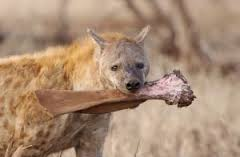
\includegraphics[width=3.33in]{images/materials_chapter/hyena}

\section{The skeleton includes all the structures that function to
absorb energy without breaking or permanently deforming, to transfer
energy from one part to another, or to store-and-release
energy}\label{the-skeleton-includes-all-the-structures-that-function-to-absorb-energy-without-breaking-or-permanently-deforming-to-transfer-energy-from-one-part-to-another-or-to-store-and-release-energy}

Most people (even many biologists!) think only of the bones when they
think of the skeleton but skeletal structures include any structure that
functions to support and physically protect the body and to transfer,
store, or absorb mechanical energy. For animals generally, and
vertebrates specifically, the skeleton includes the bones and other
mineralized tissues, cartilages, tendons, ligaments, the dermis of the
skin, and the connective tissues of the walls of the heart, the blood
vessels, the respiratory tubes, and other fluid filled tubes in the
body. Even fluids can sometimes act as skeletal elements (a hydrostatic,
or hydrostatic skeleton). And, while the bones of vertebrates are part
of the skeleton, as organs, the bones have other, non-skeletal,
functions, for example Ca\(^{2+}\) and PO\(_4^{3-}\) homeostasis, the
storage of fatty acids, and the site of the development of blood cells.
In plants, all plant cell walls act as skeletons at the cell level but
certain cells organize into distinct skeletal tissues, including
collenchyma cells in growing parts of the plant, sclerenchyma cells
called fibers, and xylem cells (including the wood in woody plants).

\begin{figure}
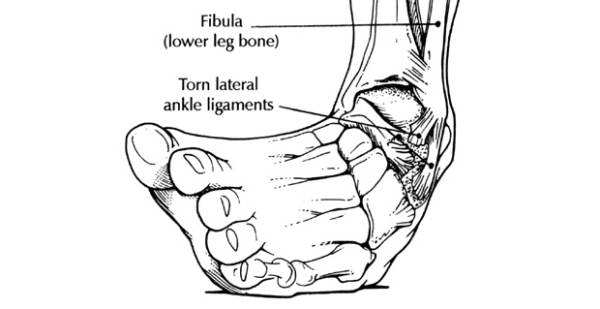
\includegraphics[width=8.33in]{images/materials_chapter/inversion} \caption{Inverted ankle joint}\label{fig:unnamed-chunk-2}
\end{figure}

A vertebrate skeleton has to do lots of things. Hyena's crush the bones
of scavenged prey to get to the fatty marrow inside. When crushing a
bone, the hyena's teeth, mandible (the bone of the lower jaw), and
maxilla (a bone of the upper jaw) need to transfer the force of muscle
contraction to crack the prey bone. Imagine if hyena teeth were made of
rubber, like a solid rubber ball. When biting bone, their teeth would
simply be squished (or \textbf{compressed}). Instead the bones of the
jaw and the teeth need to \emph{resist} deformation, or shape change, in
order to transmit the force.

\begin{figure}
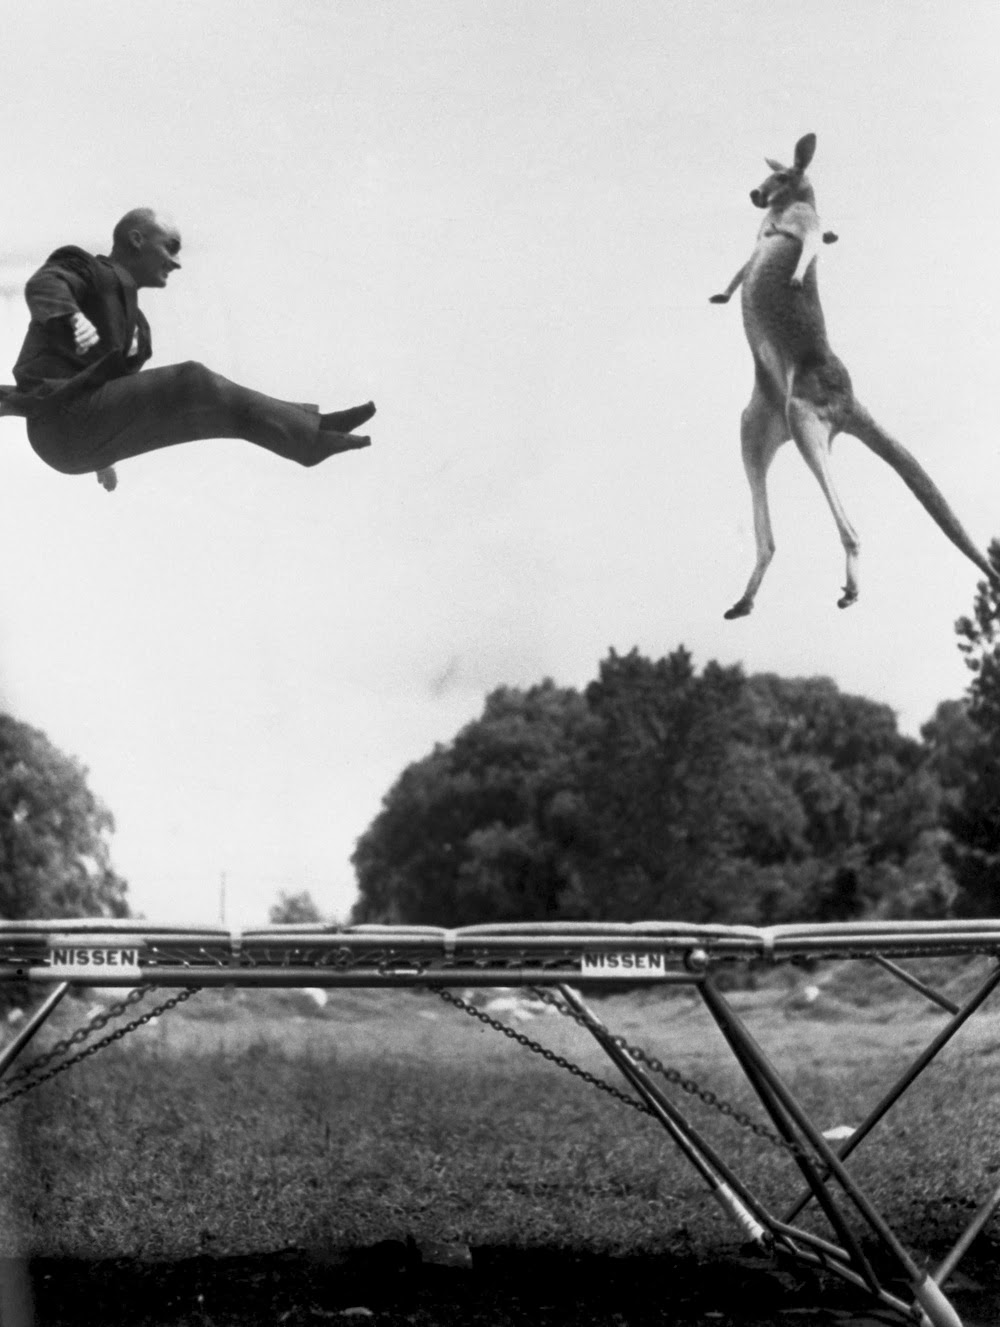
\includegraphics[width=13.89in]{images/materials_chapter/trampoline} \caption{Some tendons or ligaments act like springs}\label{fig:unnamed-chunk-3}
\end{figure}

Unlike humans, most vertebrates run on uneven surfaces filled with
rocks, roots, and small depressions and mounds. Landing on an uneven
surface will frequently put the ankle joint into bending, which applies
a force that stretches ligaments on the convex side of the bent ankle
(figure\textasciitilde{}\ref{fig:inversion}). A tight (difficult to
stretch) ligament inhibits excessive bending and thus maintains joint
stability. But in addition to be unstretchy, the ligament needs to be
tough, to keep from tearing.

An under-appreciated function of the vertebrate skeleton, especially in
introductory textbooks, is the ability of some skeletal structure to act
like a spring. Squash or stretch a spring and it springs back to its
starting length and this spring can be used to \textbf{do work} on
something, such as launching a man, or a kangaroo, against gravity. In
the vertebrate body, the skeleton of many structures act like springs
and are used to reduce the energy cost of activity, such as hopping in
kangaroos. Unlike skeletal structures used for transmitting forces or
resisting deformations, structures that act like springs should be
easily stretch or squashed.

The ability of a structure to resist stretching, or bending, or breaking
is a function of both the geometry of the structure (its size and shape)
and of the material in the structure. In this chapter, we will focus on
the latter -- the \textbf{material properties}.

\section{Skeletons are loaded by external
forces}\label{skeletons-are-loaded-by-external-forces}

We use the term \textbf{load} when we say that a pressure (or force) is
applied on an object. When we stand, our femur is loaded by the weight
of our upper body pushing down onto the femur and the earth pushing back
up. Loads come in differ flavors, or \textbf{loading environments}:

\begin{figure}
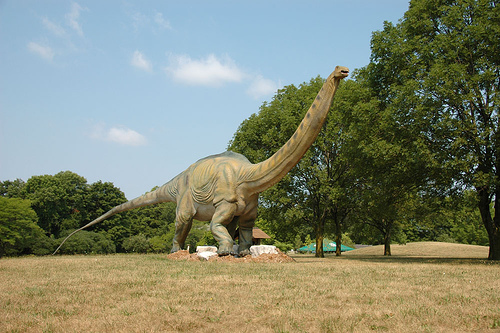
\includegraphics[width=6.94in]{images/materials_chapter/apatosaurus} \caption{Apatosaurus}\label{fig:unnamed-chunk-4}
\end{figure}

\begin{figure}
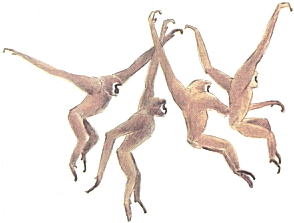
\includegraphics[width=4.08in]{images/materials_chapter/gibbon} \caption{Gibbon brachiation}\label{fig:unnamed-chunk-5}
\end{figure}

\begin{figure}
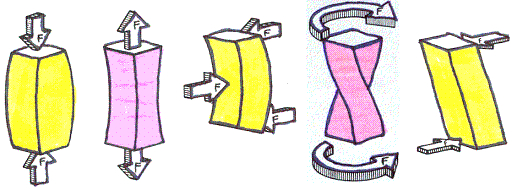
\includegraphics[width=7.11in]{images/materials_chapter/loading} \caption{Can you identify the type of loading in each of these structures?}\label{fig:unnamed-chunk-6}
\end{figure}

\begin{enumerate}
\def\labelenumi{\arabic{enumi}.}
\tightlist
\item
  \textbf{Compression} has the effect of squeezing a structure. When an
  \emph{Apatosaurus} stands, the limbs are loaded in compression because
  the weight of its (large!) body is pushing down on the limbs and a
  reactive force from the earth is pushing back up. That is, the limbs
  are squozen.
\item
  \textbf{Tension} has the effect of stretching a structure. When a
  gibbon hangs from a tree limb, its humerus, radius, humeroulnar joint,
  and wrist joint are all loaded in tension. These are being pulled
  apart because the gibbon's body weight is pulling these structures one
  way and the tree limb is pulling equally and oppositely in the other
  direction.
\item
  \textbf{Bending} has the effect of bending a structure. The vertebral
  column between the front and hind limbs of the \emph{Apatosaurus} is
  loaded in bending because the earth/limbs are pushing up at the ends
  of the column and the weight of the torso is pulling down the middle
  of the column.
\item
  \textbf{Torsion} has the effect of twisting a structure. When a
  gazelle fleeing a cheetah turns on a dime, the limbs are loaded in
  torsion because the torso is turning to the side but the ground is
  resisting the limbs from spinning.
\item
  \textbf{Shear} is the force due to materials sliding by each other.
  Shear is important in the joints where the ends of bones slide past
  each other and in the blood, where the moving blood loads the wall of
  the blood vessel in shearing.
\end{enumerate}

\section{Stress in a material is the resistance to
strain}\label{stress-in-a-material-is-the-resistance-to-strain}

When a force is applied to an object, the object deforms (often so
little that we cannot see the deformation!). How an object deforms is
really critical to its function in an organism. In order to understand
how material properties determine why some objects are very resistant to
deformation while others easily deform, or why some objects are
resistant to fracture while others are easily fractured, or why some
structures increase the efficiency of cyclical motions while others
don't, we need to separate the effects of the geometry (in general size
but sometimes shape too) of the object from the material of the object.
The size of the object is standardized by dividing by the force (\(F\))
by the cross-sectional area (\(A\)) of the object that is loaded and
dividing the change-in-length (\(\Delta L\), the deformation) by the
starting length (\(L_o\)). This results in two really fundamental
parameters:

\begin{enumerate}
\def\labelenumi{\arabic{enumi}.}
\tightlist
\item
  \textbf{strain} is the standardized deformation,
  \(\epsilon = \frac{\Delta L}{L_o}\). There are no units, that is,
  \(\epsilon\) is dimensionless
\item
  \textbf{stress} is the standardized force resisting deformation,
  \(\sigma = \frac{F}{A}\) and has SI units of
  \(\textrm{N} \cdot \textrm{m}^{-2}\), which are the units of pressure.
\end{enumerate}

\begin{figure}
\centering
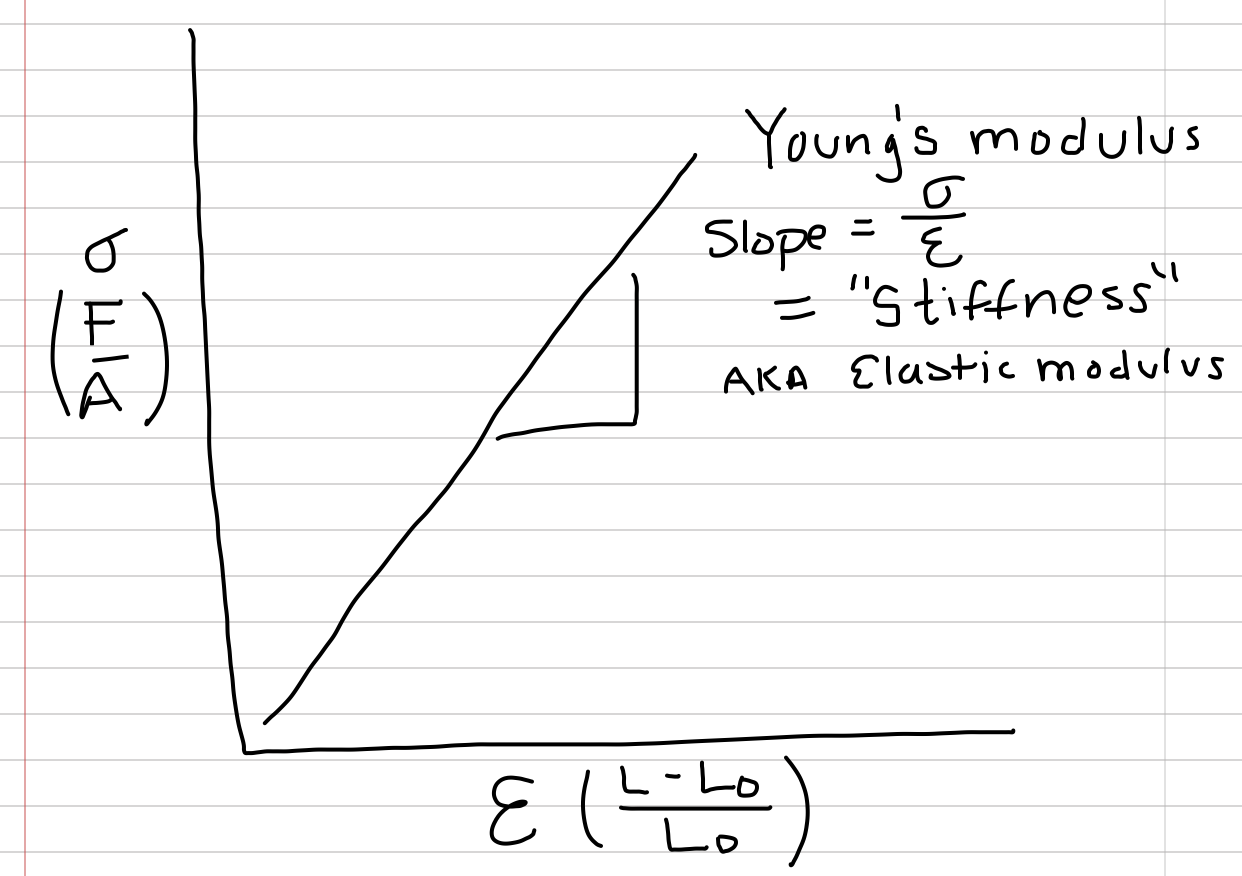
\includegraphics{images/materials_chapter/stress-strain.png}
\caption{\label{fig:unnamed-chunk-7}A somewhat idealistic stress-strain
curve}
\end{figure}

Stress is not the pressure applied to the structure but the
area-standardized reaction force of the material in response to the
external load. Stress is the reaction to strain. Or, stress is the
intrinsic resistance to strain. Deformation (strain) causes a
rearrangement of the atoms in a material. The rearranged atoms are
attracting/repelling each other in a way that will return the material
toward its starting length if the external load is removed. Stress is
this internal, standardized force due to the atoms attracting/repelling
each other. If the external load is removed from a deformed material,
there is still stress, and this stress is present until the added
attraction/repulsion force returns to their starting value. So while an
external load causes strain, strain causes stress! Importantly, all of
the loading environments described above can be applied to stress as
well, so that we use the phrase ``tensile stress''.

\begin{figure}
\centering
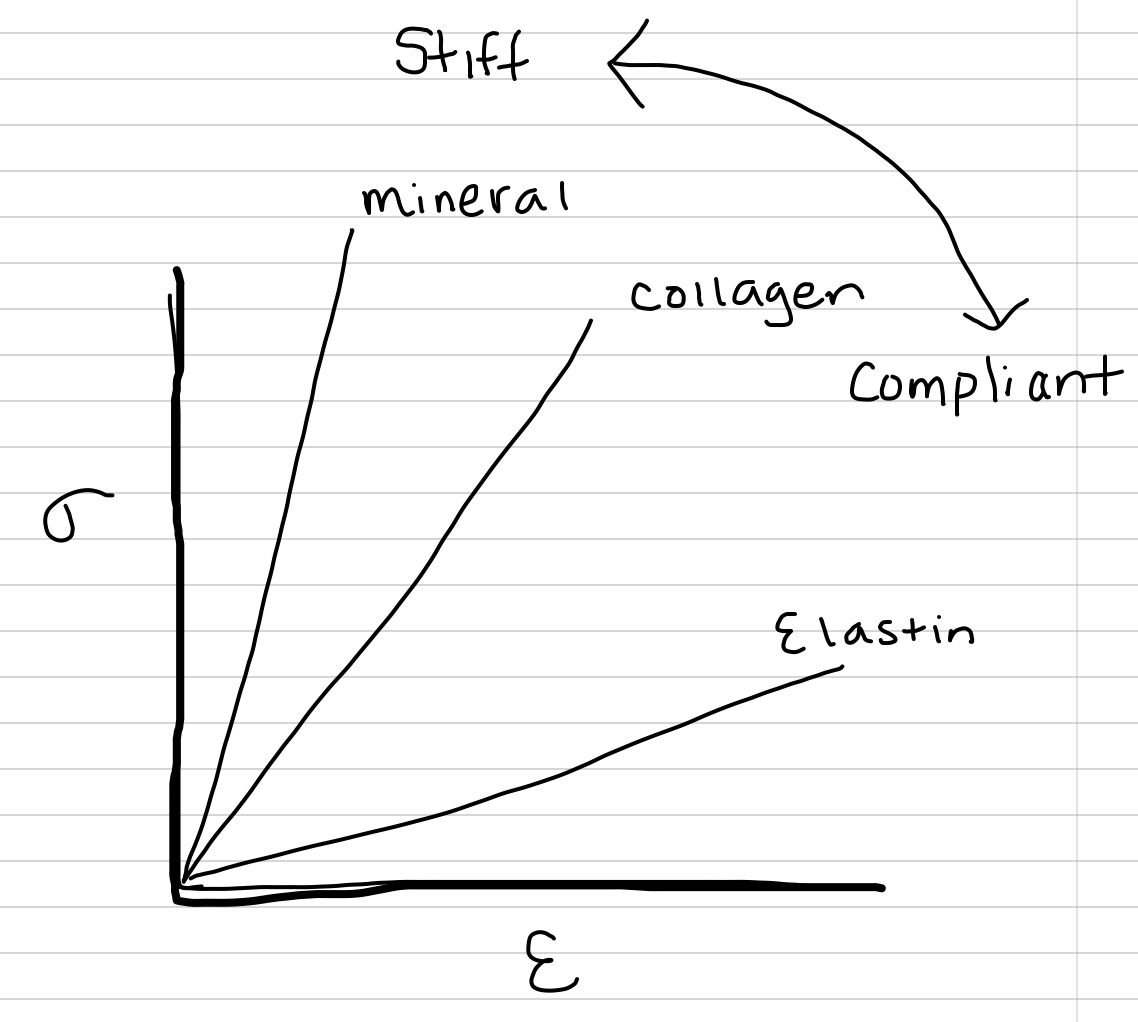
\includegraphics{images/materials_chapter/stiffness.png}
\caption{\label{fig:unnamed-chunk-8}Relative stress-strain curves for
hydroxyapatite, collagen, and elastin}
\end{figure}

This ability of a material to resist deformation is graphically shown by
the slope of a stress-strain curve, with stress (\(\sigma\)) on the
y-axis and strain \(\epsilon\) on the x-axis. This slope is called the
Elastic (or Young's) Modulus (\(E\)), or \textbf{stiffness}. Since the
curve starts at the origin (0, 0), the elastic modulus is

\[E = \frac{\sigma}{\epsilon}\]

Materials with high \(E\) (steeper slopes) are \textbf{stiff}, materials
with low \(E\) (shallower slopes) are \textbf{compliant}. Mineralized
tissue is stiff relative to a tissue with abundant collagen which is
stiff relative to a tissue with abundant elastin (we can't really test
individual proteins). Rubber in a rubber band is more compliant than
nylon used for rope.

\section{Work has to be done on a structure to deform it and generate
stress}\label{work-has-to-be-done-on-a-structure-to-deform-it-and-generate-stress}

It takes mechanical work to deform a material. Mechanical work is a form
of energy used to move an object a certain distance, \(W=Fd\). The
standard example in physics is pushing a box across a floor. But when
the weight of an \emph{Apatosaurus} deforms its femur (the bone of the
thigh), it's not the whole femur that is moving through space but the
individual atoms within the femur. All of these microscopic movements
sum up to the total amount the bone shortens under the compressive load,
\(\Delta L = L - L_o\). \(\Delta L\) is the \(d\) in the equation for
mechanical work.

\begin{figure}
\centering
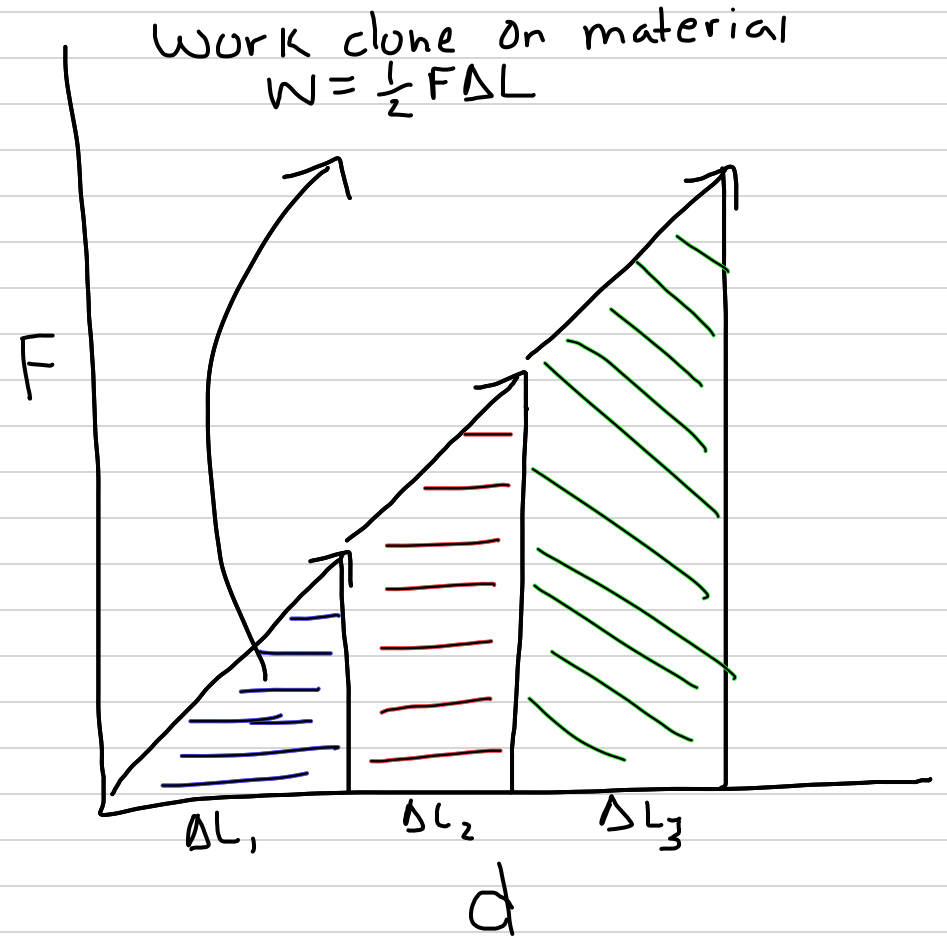
\includegraphics{images/materials_chapter/work.png}
\caption{\label{fig:unnamed-chunk-9}The area under the force-deformation
(not stress-strain!) curve at any level of deformation is the work done
to deform the material. This energy is transferred to the material.}
\end{figure}

How much work does it take to deform a structure? Imagine clamping a
cut-out piece of the wall of the aorta to a board and then clamping a
weight to the aorta and measuring \(\Delta L\). then repeat this for a
series of larger and larger weights, but instead of computing
\(\Delta L\) as the difference between the current length and starting
length, compute it as the difference between the current length and the
length with the previous, smaller weight, so
\(\Delta L_j = L_j - L_{j-1}\). An approximate measure of the additional
work done on the aorta wall to deform it this additional \(\Delta L_j\),
is \(W_j=F_j\Delta L_j\) and an approximate measure of the total work
done to deform the aorta from its starting length is \(W=\sum{W_j}\).

Additional insight is gained by plotting each of the weights (\(F_j\))
against the added deformations (\(L_j\)) using the non-standardized
measures (at this point, these are not standardized to stress and
strain). The measure of each of the components of Work, that is, the
\(W_j\), is the area of a rectangle with height \(F_j\) and width
\(\Delta L_j\). And, the total Work is an approximate measure of the
area under the curve connecting the measured points. The more weights
one uses to measure this line, the closer the approximate measure of
Work is to the area under the curve. The area under the curve is the
actual work done on the aorta wall. If this curve is a straight line,
the Work to deform the aorta is \(W=\frac{1}{2}F \Delta L\).

\section{Materials absorb strain
energy}\label{materials-absorb-strain-energy}

\begin{figure}
\centering
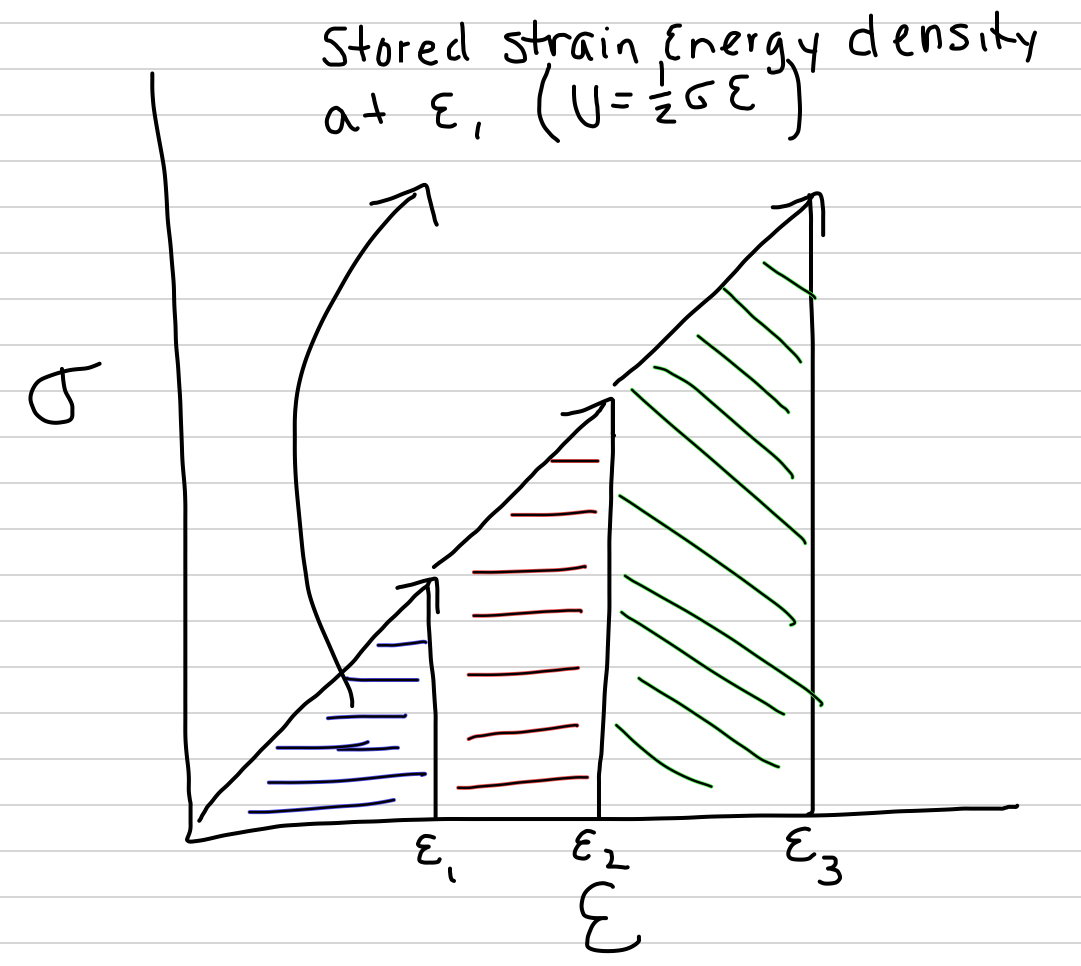
\includegraphics{images/materials_chapter/strain_energy_density.png}
\caption{\label{fig:unnamed-chunk-10}The area under the stress-strain curve
at any level of deformation is the strain-energy density (the strain
energy per unit volume) that is stored.}
\end{figure}

Doing work on a structure transfers energy into the structure. This
absorbed energy rearranges the atoms in the material. Or, we can think
of these rearranged atoms as absorbing or storing the energy. This
stored energy is known as \textbf{strain energy}. The magnitude of the
strain energy will be a function of both the geometry of the structure
and the type of material in the structure. So, to remove the influence
of geometry on this measure, we used the scaled force and deformation,
\(\sigma\) and \(\epsilon\). For a straight stress-strain curve, this
standardized energy is

\[U = \frac{1}{2} \sigma \epsilon\]

Substitute in the equations for stress and strain and this standardized
energy is

\[U=\frac{1}{2} \frac{F \Delta L}{A L_o}\]

The numerator of this equation is the mechanical work done on the
object, which is also the strain energy absorbed by the material. The
denominator is the volume of the starting object. Consequently, \(U\) is
volume-standardized strain energy, or \textbf{strain energy density}
(this is the energy stored per unit volume in analogy to density, which
is the mass per unit volume).

\section{Stored strain energy can do
work}\label{stored-strain-energy-can-do-work}

\begin{figure}
\centering
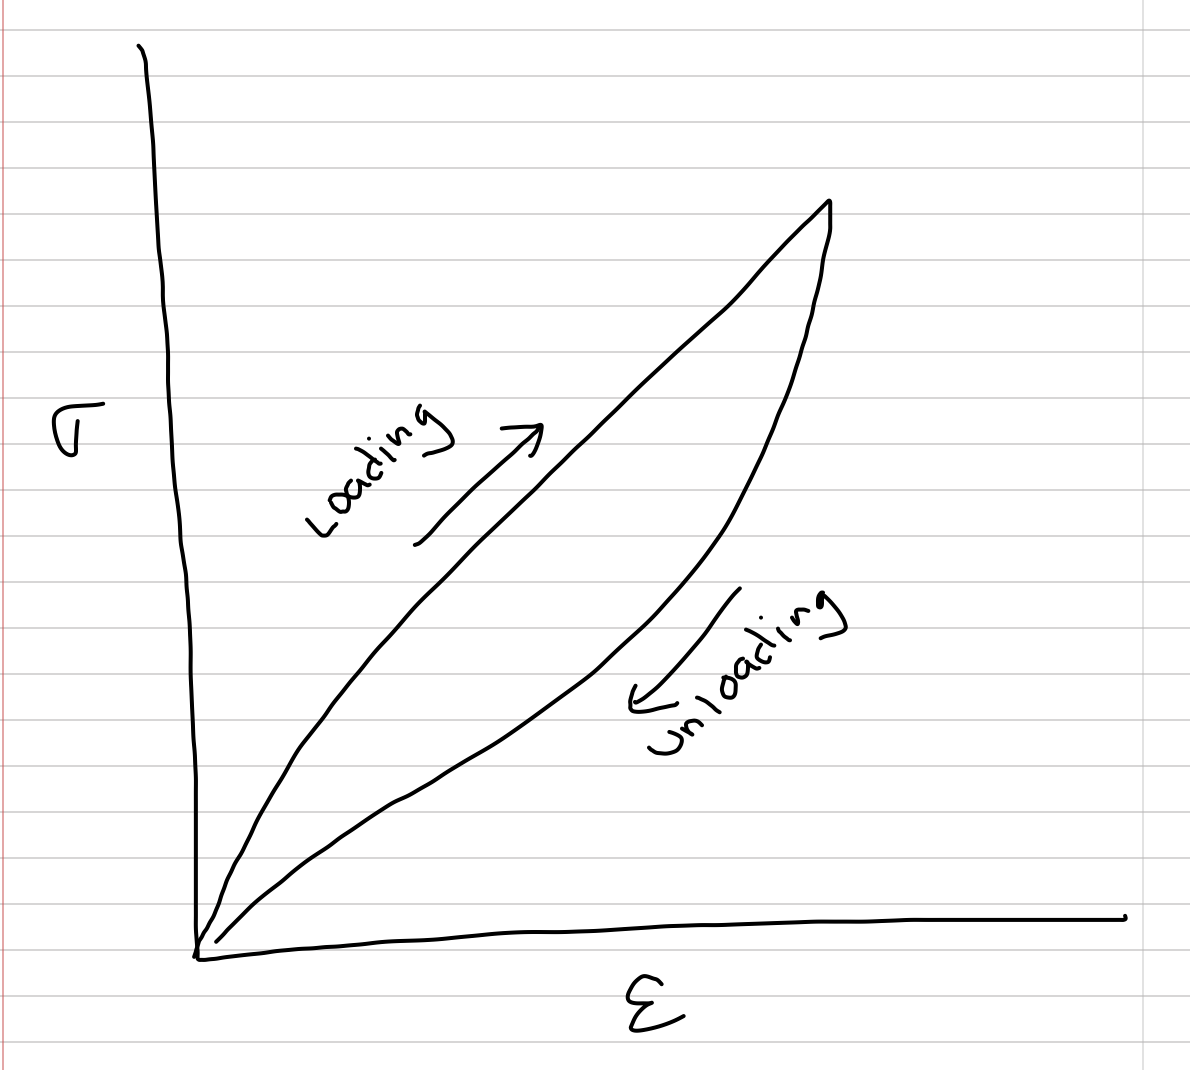
\includegraphics{images/materials_chapter/elastic_energy_storage_1.png}
\caption{\label{fig:unnamed-chunk-11}The loading curve is the behavior while
a material is being deformed by some load. The unloading curve is the
behavior when the load is removed.}
\end{figure}

If the external load is removed, the stored strain energy does work on
the surrounding material, moving the atoms back toward their starting
arrangement. In an \textbf{elastic} material, which includes most
biological materials that aren't fluid, the starting length is
completely recovered. If the surrounding material includes an another
object, some of the stored energy is transferred into that object,
typically as kinetic energy (if the object is put into motion). This
\textbf{storage and release of elastic strain energy} has profound
implications for both human engineering and for animal function. For
human-engineering, think of sling-shot. Energy from moving limbs is
transferred into the rubber material of the sling as strain energy. The
strain energy is used to return the sling to its starting length and the
energy of this return motion is used to shoot a rock. Animal bodies are
full of structures that store and release elastic strain energy. For
example, during lung ventilation in mammals, our thorax cycles between
inspiration (the inhale) and expiration (the exhale). Contraction of the
diaphragm muscle powers inspiration: the diaphragm contracts, the
thoracic volume increases, which depresses alveolar air pressure, which
sucks air into the alveoli through an open mouth and nose. The expanded
thoracic wall and lung itself store elastic strain energy. When the
diaphragm relaxes, this stored strain energy powers expiration. The
total energetic cost of ventilation is markedly reduced because of the
ability of thoracic tissues to store and release elastic strain energy.

\section{The work that a strained material can do is always less than
the work done to deform the
material}\label{the-work-that-a-strained-material-can-do-is-always-less-than-the-work-done-to-deform-the-material}

\begin{figure}
\centering
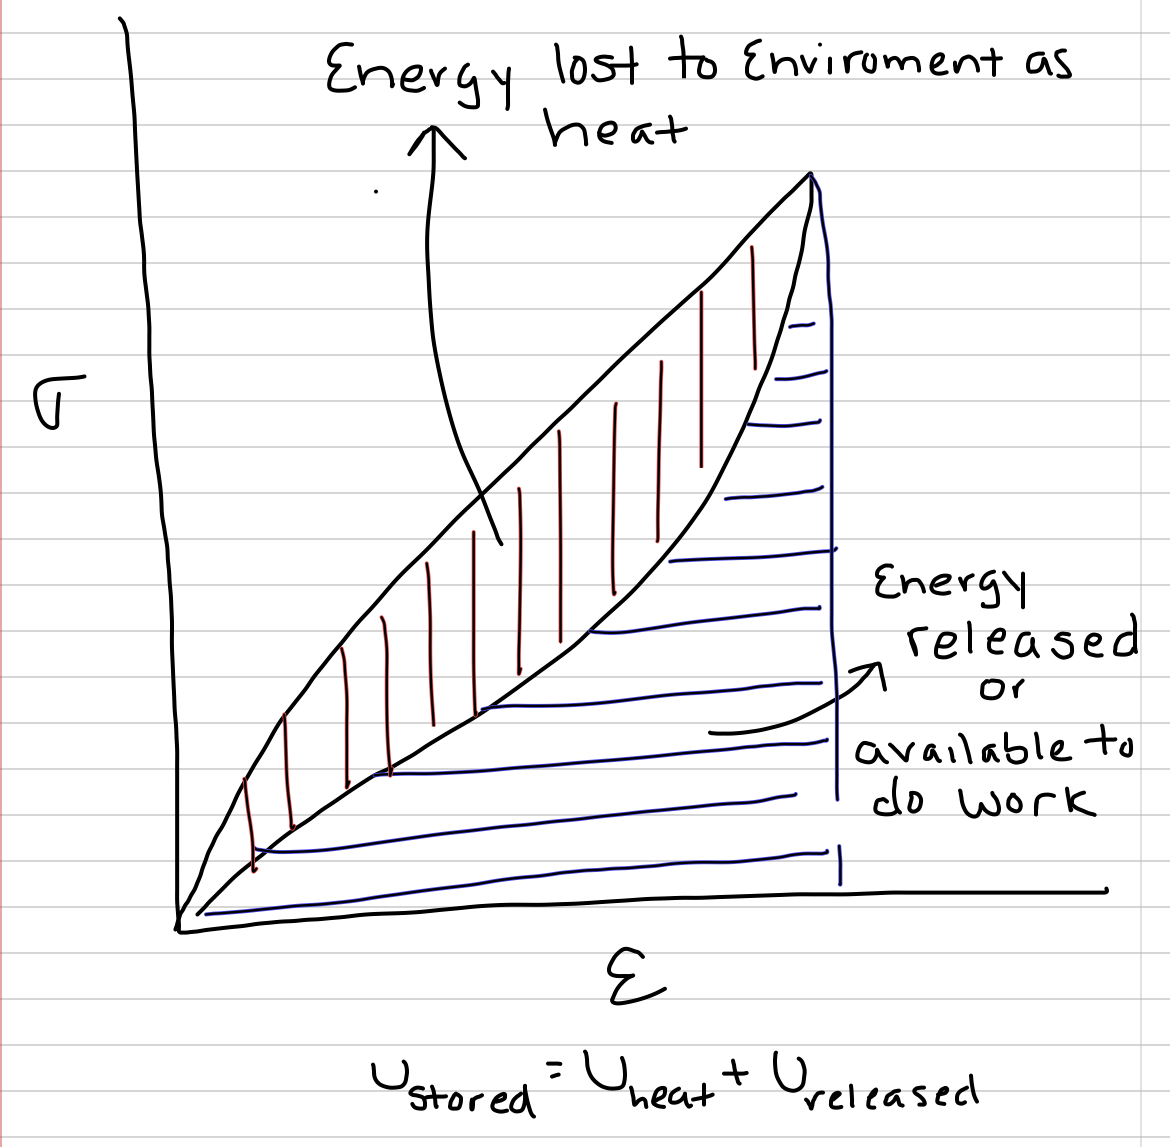
\includegraphics{images/materials_chapter/elastic_energy_storage_2.png}
\caption{\label{fig:unnamed-chunk-12}The total area under the loading curve
is the stored elastic strain energy density. The area under the
unloading curve is the fraction of stored elastic strain energy density
that is returned, or available to do work. The area between the two
curves is the fraction of stored elastic strain energy density that is
lost to the environment as heat}
\end{figure}

The stress-strain curve measured while unloading a material is always
depressed relative to the curve measured while loading the material. The
area under the loading curve is volume-standardized work done on the
material (so the actual work is this number times the volume of the
material). This volume-standardized work is equal to the stored
strain-energy density. The area under the unloading curve is the
fraction of the stored strain-energy density that is available for doing
mechanical work on surrounding matter. This released elastic strain
energy is always less than the stored elastic strain energy. The
difference between the stored energy and the released energy is
transferred to the environment as heat.

\section{Material Properties determine if a tissue is good at absorbing
strain energy without breaking or storing and releasing lots of elastic
strain
energy}\label{material-properties-determine-if-a-tissue-is-good-at-absorbing-strain-energy-without-breaking-or-storing-and-releasing-lots-of-elastic-strain-energy}

\begin{figure}
\centering
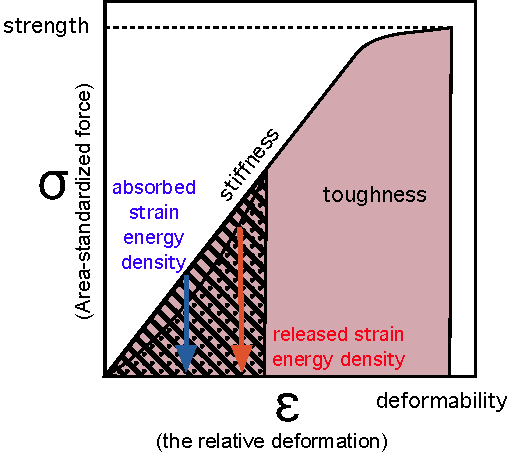
\includegraphics{images/materials_chapter/stress_strain_I.pdf}
\caption{\label{fig:unnamed-chunk-13}Illustration of material properties.
Strength is the maximum stress without failure. Deformability is the
maximum strain without failure. Stiffness is the elastic modulus and is
the slope of the curve. Toughness is the area in red. The input
(absorbed) strain energy density is the hatched area. The output
(released) strain energy density is the dotted area. The hatched area
without dots is the amount of heat produced when the elastic material
returns to its starting length. Resilience is the ratio of output to
input strain energy density.}
\end{figure}

These material properties are

\begin{enumerate}
\def\labelenumi{\arabic{enumi}.}
\tightlist
\item
  \textbf{Stiffness}, aka the Modulus of Elasticity, the Elastic
  Modulus, or Young's Modulus, is the slope of the stress strain curve,
  which is \(E = \frac{\sigma}{\epsilon}\) for a material with a linear
  curve. \(E\) is a measure of the resistance to deformation. I usually
  just refer to this measure as the material's \textbf{stiffness}. The
  more force it takes to deform a material a certain amount, the higher
  the elastic modulus. Or from the view of the material, the elastic
  modulus is high if only a small strain creates a high stress. A
  material with a high elastic modulus is \textbf{stiff}. The opposite,
  a material with a low elastic modulus, is \textbf{compliant}.
  Compliant materials are easily stretched or squished.
\item
  \textbf{Strength}, or breaking strength, or tensile strength (if in
  tension), is the maximum stress that a material can resist without
  \textbf{failing}, or breaking. A \textbf{strong} material can
  withstand high stress before failure. The opposite is \textbf{weak}.
\item
  \textbf{Deformability} is the strain of the material at failure. If
  the material is in tension, this is \textbf{extensability}. All highly
  deformable materials are compliant but not all compliant materials are
  highly deformable.
\item
  \textbf{Toughness}, T, is the strain energy density at failure.
  Materials that can absorb lots of strain energy are tough. The
  opposite is brittle. Stiff materials tend to be brittle. More
  compliant (but not too compliant!) materials tend to be tough. Bones
  used for support (and the wood of tree trunks) must be tough in
  addition to being strong.
\item
  \textbf{Resilience}, R, is the percent of the total absorbed strain
  energy that can be used to do work and so is the ratio of the released
  strain energy (\(U_{out}\), the area under the unloading curve) to the
  total absorbed strain energy (\(U_{in}\), the area under the loading
  curve). This ratio is always less than one (otherwise a ball made of a
  material with a resilience of one could bounce forever!). The ability
  of a tissue to store-and-release elastic strain energy is a function
  of both resilience and compliance. Collagen and elastin are both very
  resilient but collagen is also much stiffer than elastin.
\end{enumerate}

\chapter{Gearing Ratios}\label{gearing-ratios}

\section{Gears control an output force or displacement or
speed}\label{gears-control-an-output-force-or-displacement-or-speed}

Everyone is familiar with gears in human engineered devices. A gear is a
device for controlling an output force or displacement or speed given a
certain input force. In a bicycle, we apply an input force to the pedal
and crank and get an output force of the rear tire pushing the ground
rearward, causing the bike to move forward. In a geared bike, a low gear
is used for generating large output force -- for large accelerations or
for climbing a steep hill. A high gear is used at high speed on flat or
descending road. This high speed is achieved because the rear wheel is
turning many times for each rotation of the crank. This turning is the
output displacement. High gear results in high output displacement. The
more displacement per unit time (say the time it takes to rotate the
crank once), the higher the speed. There is a trade-off in gears -- a
low gear generates high highput force but low displacement. A high gear
results in high displacement but low output force.

\section{Vertebrate musculoskeletal systems are
geared}\label{vertebrate-musculoskeletal-systems-are-geared}

\begin{figure}
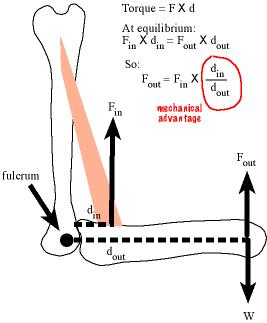
\includegraphics[width=3.71in]{images/gear_chapter/mechanical_advantage} \caption{Mechanical advantage.}\label{fig:gearing1}
\end{figure}

What may be surprising is that vertebrate musculoskeletal systems are
geared. Consider figure \ref{fig:gearing1}, which is a cartoon of a
biceps muscle, a humerus and radius being used to move (or resist being
moved by) a load. Here, the load is an invisible coffee mug that weighs
\(W\). My biceps muscle doesn't directly lift the coffee mug but instead
the biceps-humerus-radius system generates an output force \(F_{out}\)
to hold or move the mug. The force from the contracting biceps muscle is
the input force \(F_{in}\). The output force is the useful force. It is
what is used to pick up and move stuff. How much (input) force does my
biceps need to generate to hold the coffee mug?

To answer this, we need the concept of torque. A \textbf{torque} (or
\textbf{moment}), is a force that causes a rotation about an axis
through a center of rotation (a \textbf{fulcrum}) and is equal to the
force times the distance between the application of the force and the
center of rotation.\footnote{\(M = F \times d\)}. For example, if I
apply a force to a wrench, the torque is the force times the length of
the handle, since I apply the force at the end of the handle and the
center of rotation is the center of the bolt. The distance (\(d\)) is
known as the moment arm or lever arm.\footnote{A ``moment'' is used for
  other concepts in math and science that are a function of some value
  multiplied by a distance to a center. And, if the distance is squared,
  it is a second moment. A cubed distance is a third moment.}

The radius rotates around an axis that is perpendicular to the plane of
the image and pierces the joint at the center of rotation (fulcrum). The
load is applying a torque on the fulcrum. The action of the torque is to
rotate the forearm about this axis in a clockwise direction, which
increases the joint angle and lengthens the biceps muscle. A contracting
biceps muscle is also applying a torque on the fulcrum. The action of
this torque is the rotation of the forearm in a counterclockwise motion.

If the output force balances the weight of the coffee mug then the input
torque must equal the output torque, or

\[F_{out}d_{out} = F_{in}d_{in}\] which we can re-arrange to solve for
output force

\[F_{out}= F_{in}\frac{d_{in}}{d_{out}}\]

A bigger input force generates a bigger output force. A longer input
moment arm generates a bigger output force. A smaller output moment arm
generates a bigger output force. Consider how these might vary both
within an individual and among individuals or species. The input force
is the force generated by the muscle. Individuals can control the
magnitude of this force and of course there will be variation among
individuals and species due ot the size of the muscle, the geometry of
the fibers, and the proportions of the different fiber types. The input
moment arm is the distance of the insertion of the muscle from the
center of rotation in the joint. An individual certainly cannot control
this. But there is variation among individuals and among species. The
output moment arm is whatever we want it to be. If we want to compute
the output force applied 4 cm from the center of rotation then we set
the output moment arm to 4 cm. If we consider the output force at the
hand, then an individual cannot vary the output moment arm -- its simply
the length of the forearm. But there will be variation among individuals
and among species.

So the input force is a function of the strength of the muscle but an
output force is a function of how the muscle is geared, or the gear
ratio. This ratio is the length of the input moment arm relative to the
length of the output moment arm, which is known as the
\textbf{mechanical advantage}.\footnote{\(MA=\frac{d_{in}}{d_{out}}\)}
Somewhat confusingly, a high gear ratio is a low gear while a low gear
ratio is a high gear.

\begin{figure}
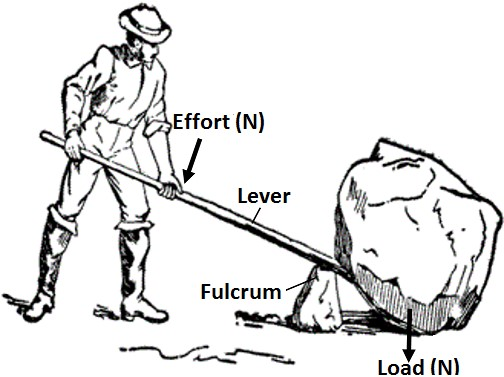
\includegraphics[width=7in]{images/gear_chapter/leverage} \caption{Levers.}\label{fig:rock1}
\end{figure}

Humans have used levers to create a mechanical advantage to move heavy
stones for thousands of years (figure \ref{fig:rock1}. In the mechanical
system created by the lever, the input lever arm (the distance from the
applied force by the man to the fulcrum) is much larger than the output
lever arm (the distance from the load to the fulcrum), so the mechanical
advantage is much greater than one. The lever magnifies the input force
and the man can move a much larger rock than he could by simply lifting
it directly.

By contrast, the mechanical advantage in the biceps-humerus-radius
system above is much smaller than one -- our maximum output force is
much less than our maximum muscle contractile force. That is, this
system is high geared. One advantage of the high gear is that we get
large displacement (motion about the joint) with only a small shortening
of the muscle. This is the displacement advantage, which is simply the
reciprocal of the mechanical advantage.\footnote{\(DA = \frac{d_{out}}{d_{in}}\)}

\begin{figure}
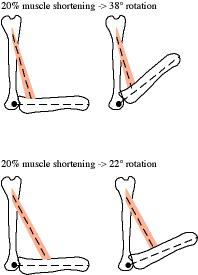
\includegraphics[width=2.75in]{images/gear_chapter/velocity_advantage} \caption{Displacement advantage.}\label{fig:velocity1}
\end{figure}

Figure \ref{fig:velocity1} shows why a high mechanical advantage and
displacment trade-off in a geared system. The biceps-humerus-radius
system in the top panel has a smaller mechanical advantage than that in
the bottom panel because the muscle inserts closer to the joint, that is
the input moment arm is shorter so \(MA\) is smaller. The right side
figures show the movement that occurs with 20\% shortening of the muscle
(the length of the muscle in the right side figures are literally 20\%
shorter than those in the left side). The radius in the top panel, with
the smaller \(MA\), rotated 38 degrees while the radius in the bottom
panel, with the larger \(MA\), only rotated 22 degrees. The smaller
input moment arm in the top system increased the displacement advantage.


\end{document}
